\documentclass[11.5pt]{beamer}

\usetheme[progressbar=frametitle]{metropolis}
\usepackage{appendixnumberbeamer}
\usepackage{booktabs}
\usepackage[scale=2]{ccicons}

\usepackage{pgfplots}
\usepgfplotslibrary{dateplot}

\usepackage{xspace}
\usepackage{graphicx}
\usepackage{amsmath}
\usepackage{enumerate}
\usepackage{enumitem}
\usepackage{amssymb}
\usepackage{color}
\usepackage{multicol}
\usepackage{bm}
\usepackage{tikz}
\usetikzlibrary{arrows,shapes}
\usepackage[ruled]{algorithm2e}
\usepackage{animate}

\setlist[itemize,1]{label=$\bullet$}
\setlist[itemize,2]{label=$\triangleright$}
\setlist[itemize,3]{label=$\diamond$}
\setlist[itemize,4]{label=$\checkmark$}

\newcommand{\pluseq}{\mathrel{+}=}
\newcommand{\asteq}{\mathrel{*}=}
\newcommand{\norm}[1]{\left\lVert#1\right\rVert}
\newcommand{\Rdom}{\mathbb{R}}
\newcommand{\bx}{\bm{x}}
\newcommand{\themename}{\textbf{\textsc{metropolis}}\xspace}
\newcommand{\argmin}[1]{\underset{#1}{\operatorname*{arg\,min\,}}}
\newcommand{\argmax}[1]{\underset{#1}{\operatorname*{arg\,max\,}}}
\newcommand{\undermin}[1]{\underset{#1}{\operatorname*{min\,}}}
\title{EM Algorithm}
\subtitle{Chapter 9, Statistical learning methods}
\date{\today}
\author{Yu Hao}
\institute{NaMI, Tongji University}
% \titlegraphic{\hfill
\includegraphics[height=1.5cm]{Tongji_University.png}}

\begin{document}
\tikzstyle{every picture}+=[remember picture]
\everymath{\displaystyle}

\maketitle

\begin{frame}{Table of contents}
\setbeamertemplate{section in toc}[sections numbered]
\tableofcontents[hideallsubsections]
\end{frame}

\section{K-means}
\begin{frame}{K-means recap}
\begin{itemize}
	\item Randomly initialize $K$ centers 
	\begin{itemize}
		\item $\bm{\mu}^{(0)}=\bm{\mu}_{1}^{(0)},\ldots,\bm{\mu}_{K}^{(0)}$
	\end{itemize}
	\item \textcolor{red}{Classify:} Assign each point $j\in{\left\{ 1,\ldots,N \right\}}$ to nearest center:
	\begin{itemize}
		\item $C^{(t)}(j) \leftarrow \argmin{i} \norm{\bm{\mu}_i-\bm{x}_j}^2$
	\end{itemize}
	\item \textcolor{red}{Recenter:} $\bm{\mu}_i$ becomes centroid of its points
	\begin{itemize}
		\item $\bm{\mu}_{i}^{(t+1)}\leftarrow\argmin{\bm{\mu}}\sum_{j: C(j)=i} \norm{\bm{\mu}-\bm{x}_{j}}^2$
		\item Equivalent to $\bm{\mu}_i \leftarrow$ average of its points!
	\end{itemize}
\end{itemize}
\end{frame}

\begin{frame}{What is K-means optimizing?}
\begin{itemize}
	\item Potential function $F(\bm{\mu},C)$ of centers $\bm{\mu}$ and point allocations $C$:
	\begin{equation}
	F(\bm{\mu},C)=\sum_{j=1}^{N} \norm{\bm{\mu}_{C(j)}-\bm{x}_j}^2
	\end{equation}
	\item Optimal K-means:
	\begin{itemize}
		\item $\undermin{\bm{\mu}}\undermin{C}F(\bm{\mu},C)$
	\end{itemize}
\end{itemize}
\end{frame}

\begin{frame}{K-means algorithm}
\tikzstyle{na} = [baseline=-.5ex]
\begin{itemize}
	\item Optimize potential function:
	\begin{equation}
	\undermin{\bm{\mu}}\undermin{C}F(\bm{\mu},C)=\undermin{\bm{\mu}}\undermin{C}\sum_{i=1}^{K}\sum_{j:C(j)=i}\norm{\bm{\mu}_i-\bm{x}_i}^2
	\end{equation}
	\item \textcolor{red}{K-means algorithm:}
	\begin{itemize}
		\only<1>{
		\item \textcolor{red}{(1)} Fix $\bm{\mu}$, optimize $C$
		\begin{equation} \nonumber
		\undermin{C}\sum_{j=1}^{N}\norm{\bm{\mu}_{C(j)}-x_j}^2=\sum_{j=1}^{N}
		\tikz[baseline]{\node[fill=red!20,anchor=base,ellipse](e1){$\undermin{C(j)}\norm{\bm{\mu}_{C(j)}-\bm{x}_j}^2$};}
		\end{equation}
		Exactly first step: assign each point to the \textcolor{red}{nearest} \tikz[na] \node[coordinate] (n1) {}; cluster center
		\begin{tikzpicture}[overlay]
		\path[->]<1-> (n1) edge [bend right] (e1);
		\end{tikzpicture}
		}
		\only<2>{
		\item \textcolor{red}{(2)} Fix $C$, optimize $\bm{\mu}$
		\begin{equation} \nonumber
		\undermin{\bm{\mu}}\sum_{i=1}^{K}\sum_{j:C(j)=i}\norm{\bm{\mu}_i-\bm{x}_j}^2=\sum_{i}^{K}
		\tikz[baseline]{\node[fill=red!20,anchor=base,](e2){$\undermin{\bm{\mu}_i}\sum_{j:C(j)=i}\norm{\bm{\mu}_{i}-\bm{x}_j}^2$};}
		\end{equation}
		Exactly second step: \textcolor{red}{average of points} \tikz[na] \node[coordinate] (n2) {}; in cluster $i$
		\begin{tikzpicture}[overlay]
		\path[->]<1-> (n2) edge [bend right=120] (e2);
		\end{tikzpicture}
		}
		\only<3>{
		\item \textcolor{red}{(1)} Fix $\bm{\mu}$, optimize $C$ \qquad \textbf{\textcolor{red}{Expectation step}}
		\item \textcolor{red}{(2)} Fix $C$, optimize $\bm{\mu}$ \qquad \textbf{\textcolor{red}{Maximization step}}
		\item Today, we will see a generalization of this approach: \qquad \textbf{\textcolor{red}{EM algorithm}}
		}
	\end{itemize}
\end{itemize}
\end{frame}

\begin{frame}{Iterations of K-means}
\begin{figure}
\animategraphics[controls,width=7cm]{2}{kmeans_gif/}{0}{14}
\end{figure}
\end{frame}

\begin{frame}{K-means decision boundaries}
\begin{columns}[c]
\column{8cm}
\begin{figure}
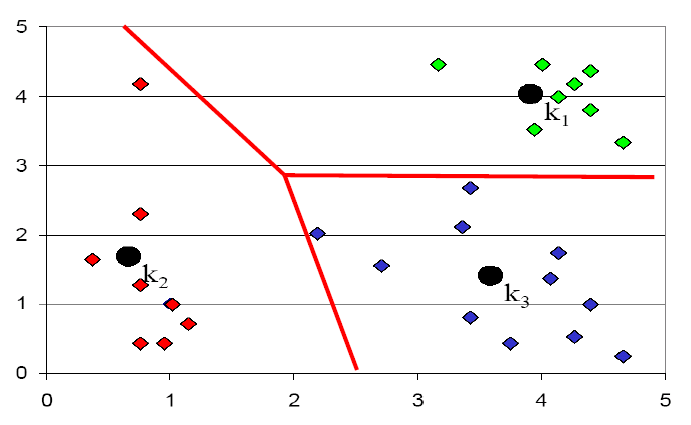
\includegraphics[width=7cm]{pics/kmean_decision_boundaries}
\end{figure}
\column{3cm}
"Linear" Decision Boundaries
\end{columns}
\begin{itemize}
	\item \textbf{\textcolor{red}{Generative Model:}}

	Assume data comes from a mixture of $K$ Gaussians distributions
	with same variance.
\end{itemize}
\end{frame}

\begin{frame}{K-means: Generative model}
\tikzstyle{na} = [baseline=-.5ex]
Mixture of $K$ Gaussians distributions: (Multi-model distribution)
\begin{columns}[c]
\column{7cm}
\begin{itemize}
	\only<1-2>{
	\item There are $K$ components
	\item Component $i$ has an associated mean vector $\bm{\mu}_i$}
	\only<2>{
	\item Each component generates data from a Gaussian with mean $\bm{\mu}_i$ and covariance matrix $\sigma^2\mathbf{I}$
	}
	\only<3-4>{
	\item Each data point is generated according to the following recipe:
	\item (1) Pick a component at random: choose component $i$ with probability $P(y=i)$
	}
	\only<4>{
	\item (2) Data point $\bm{x} \sim \mathcal{N}(\bm{\mu}_i,\sigma^2\mathbf{I})$
	}
	\only<5-6>{
	\item $p(\bm{x}|y=i) \sim \mathcal{N}(\bm{\mu}_i,\sigma^2\mathbf{I})$ \\[15pt]
	}
	\only<5>{
	\item $p(\bm{x})=\sum_{i} \textcolor{red}{p(\bm{x}|y=i)} \textcolor{blue}{P(y=i)} $
	\begin{itemize}
		\item \textcolor{red}{Mixture component}
		\item \textcolor{blue}{Mixture proportion}
	\end{itemize}
	}
	\only<6>{
	\item Gaussian Bayes Classifier:
	\begin{equation} \nonumber
	\begin{aligned}
	&\log \frac{P(y=i|\bm{x})}{P(y=j|\bm{x})} \\[6pt]
	&=\log \frac{p(\bm{x}|y=i)P(y=i)}{p(\bm{x}|y=j)P(y=j)} \\[6pt]
	&=\textcolor{red}{\bm{w}}^{T}\bm{x}
	\end{aligned}
	\end{equation}
	\item \textcolor{red}{$\bm{w}$} depends on $\bm{\mu},\sigma^2,P(y)$
	}
\end{itemize}
\column{6cm}
\begin{figure}
\only<1>{
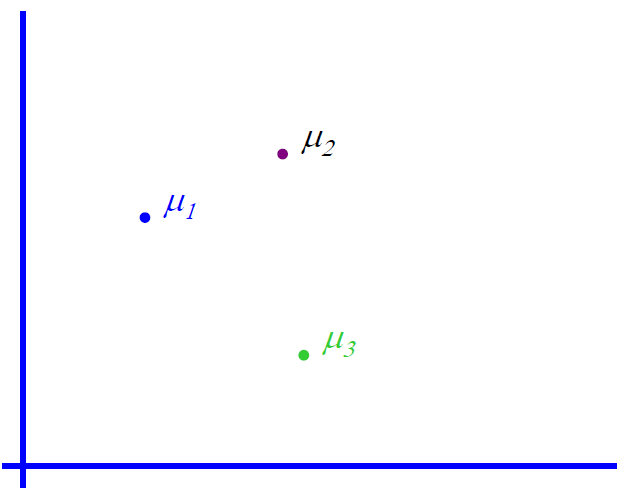
\includegraphics[width=6cm]{pics/kmeans_generative_model_1}
}
\only<2>{
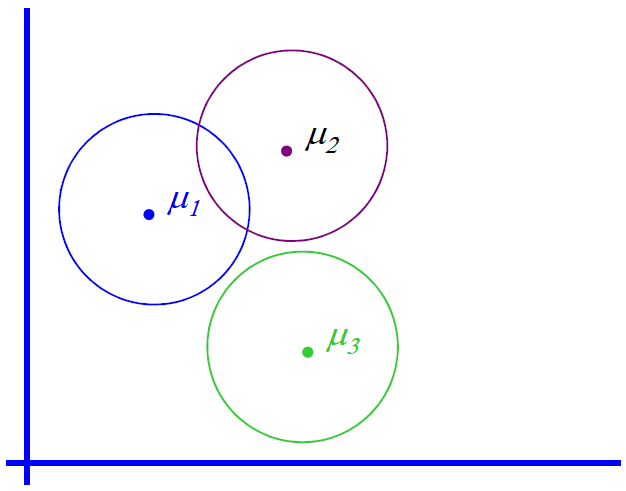
\includegraphics[width=6cm]{pics/kmeans_generative_model_2}
}
\only<3>{
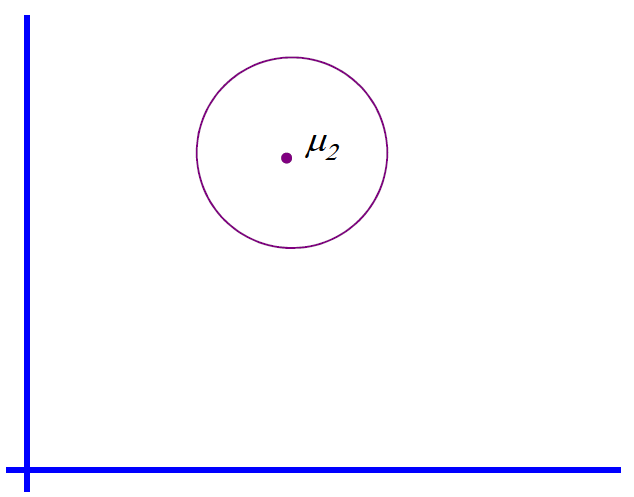
\includegraphics[width=6cm]{pics/kmeans_generative_model_3}
}
\only<4>{
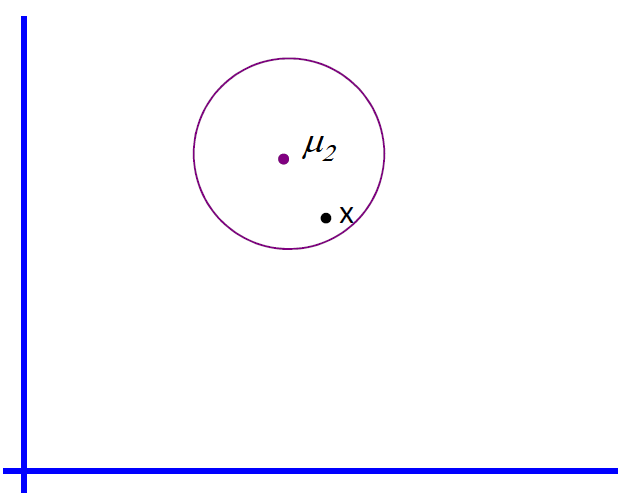
\includegraphics[width=6cm]{pics/kmeans_generative_model_4}
}
\only<5>{
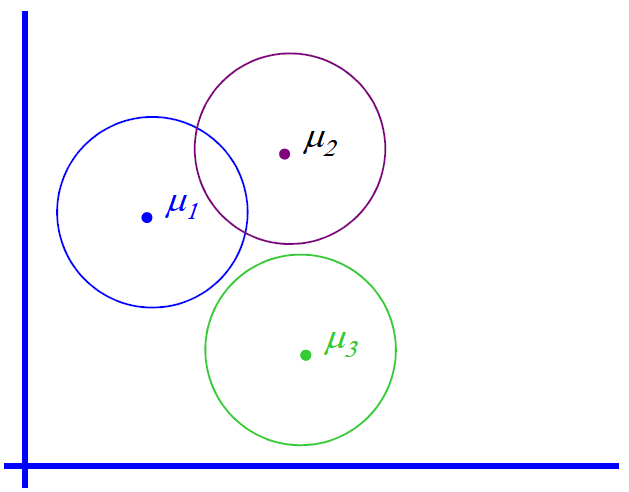
\includegraphics[width=6cm]{pics/kmeans_generative_model_5}
}
\only<6>{
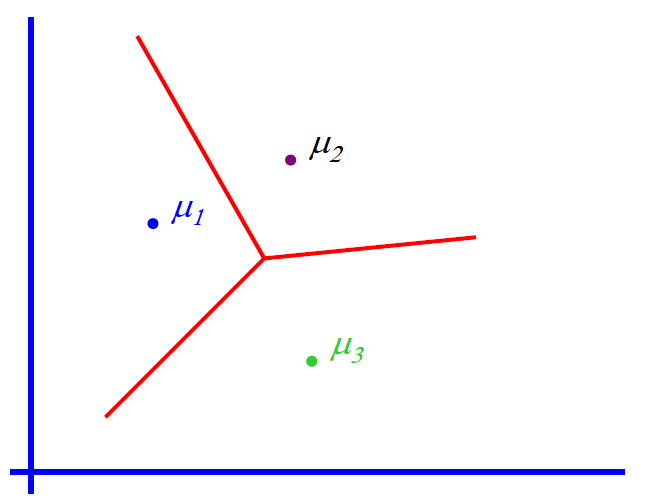
\includegraphics[width=6cm]{pics/kmeans_generative_model_6}
"Linear Decision boundary"
second-order terms cancel out
}
\end{figure}
\end{columns}
\end{frame}

\begin{frame}{K-means: MLE}
\begin{itemize}
	\only<1>{
	\item Maximum Likelihood Estimate (MLE)
	\begin{equation} \nonumber
	\argmax{\bm{\mu}, \sigma^2, P(y)}\prod_{i} P(y_i,\bm{x}_i)
	\end{equation}
	But we don't know $y_i$ is!
	}
	\only<1-2>{
	\item Maximize marginal likelihood:
	\begin{equation} \nonumber
	\begin{aligned}
	&\argmax{} \prod_{j} P(\bm{x}_j) \\
	=&\argmax{} \prod_{j}\sum_{i}^{K}P(y_j=i,\bm{x}_j) \\
	=&\argmax{} \prod_{j}\sum_{i}^{K}P(y_j=i)\textcolor{red}{p(\bm{x}_j|y_j=i)}
	\end{aligned}
	\end{equation}
	}
	\only<2>{
	\item Substitute with Gaussian distribution probability:
	\begin{equation} \nonumber
	P(y_j=i,\bm{x}_j) \propto P(y_j=i) \textcolor{red}{\exp \left[ -\frac{1}{2\sigma^2}\norm{\bm{x}_j-\bm{\mu}_i}^2 \right]}
	\end{equation}
	}
	\only<3>{
	\item If each $\bm{x}_j$ belongs to one class $C(j)$ (hard assignment), marginal likelihood:
	\begin{equation} \nonumber
	P(y_j=i)=
	\begin{cases}
	1& C(j)=i\\
	0& else
	\end{cases}
	\end{equation}
	\item Then, the log-likelihood function is
	\begin{equation} \nonumber
	\begin{aligned}
	\ln \prod_{j=1}^{N}\sum_{i=1}^{K}P(y_j=i,x_j) &\propto \ln \prod_{j=1}^{N} \exp \left[ -\frac{1}{2\sigma^2}\norm{\bm{x}_j-\bm{\mu}_{C(j)}}^2 \right] \\
	&=\sum_{j=1}^{N}-\frac{1}{2\sigma^2}\norm{\bm{x}_j-\bm{\mu}_{C(j)}}^2
	\end{aligned}
	\end{equation}
	\centering
	\textbf{\textcolor{red}{Same as K-means!}}
	}
\end{itemize}
\end{frame}

\begin{frame}{One bad case for K-means}
\begin{columns}[c]
\column{3cm}
\begin{figure}
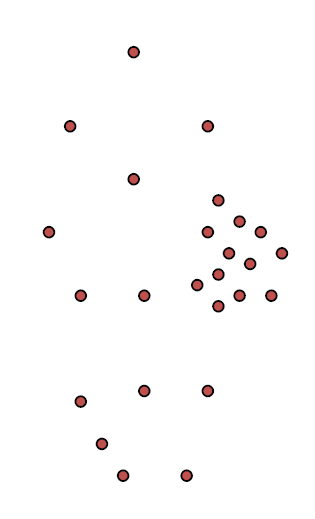
\includegraphics[width=3cm]{pics/kmeans_bad_case}
\end{figure}
\column{8cm}
\begin{itemize}
	\item CLusters may not be linear separable
	\item Clusters may overlap
	\item Some clusters may be "wider" than others
\end{itemize}
\end{columns}
\end{frame}

\section{Gaussian Mixture Model}
\begin{frame}{General GMM}
GMM-Gaussian Mixture Model (Multi-model distribution)
\begin{columns}[c]
\column{7cm}
\begin{itemize}
	\only<1>{
	\item There are $K$ components
	\item Component $i$ has an associated mean vector $\bm{\mu}_i$
	\item Each component generates data from Gaussian with mean $\bm{\mu}_i$ and covariance matrix $\Sigma_{i}$
	}
	\only<2>{
	\item Each data is generated according to the following recipe:
	\item (1) Pick a component at random: Choose component $i$ with probability $P(y=i)$
	\item (2) Data point $\bm{x} \sim \mathcal{N}(\bm{\mu}_i,\Sigma_{i})$
	}
	\only<3-4>{
	\item $p(\bm{x}|y=i)\sim \mathcal{N}(\bm{\mu}_i,\Sigma_i)$ \\[15pt]
	}
	\only<3>{
	\item $p(\bm{x})=\sum_{i} \textcolor{red}{p(\bm{x}|y=i)} \textcolor{blue}{P(y=i)} $
	\begin{itemize}
		\item \textcolor{red}{Mixture component}
		\item \textcolor{blue}{Mixture proportion}
	\end{itemize}
	}
	\only<4>{
	\item Gaussian Bayes Classifier:
	\begin{equation} \nonumber
	\begin{aligned}
	&\log \frac{P(y=i|\bm{x})}{P(y=j|\bm{x})} \\[6pt]
	&=\log \frac{p(\bm{x}|y=i)P(y=i)}{p(\bm{x}|y=j)P(y=j)} \\[6pt]
	&=\bm{x}^T\textcolor{red}{\mathbf{W}}\bm{x}+\textcolor{red}{\bm{w}}^T\bm{x}
	\end{aligned}
	\end{equation}
	\item \textcolor{red}{$\mathbf{W},\bm{w}$} depends on $\bm{\mu},\Sigma,P(y)$
	}
\end{itemize}

\column{6cm}
\begin{figure}
\only<1-3>{
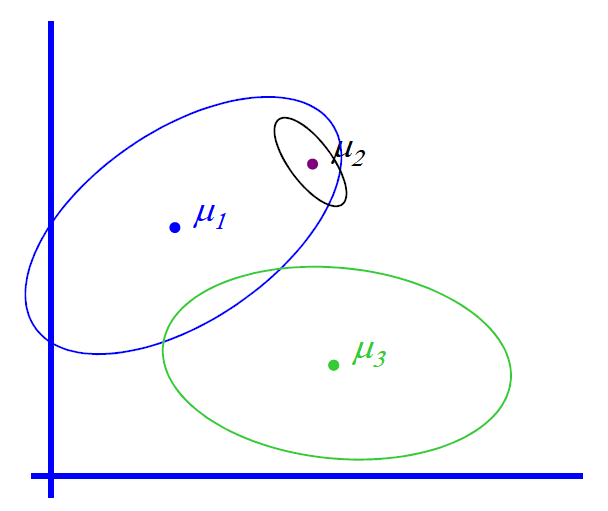
\includegraphics[width=6cm]{pics/general_gmm_1}	
}
\only<4>{
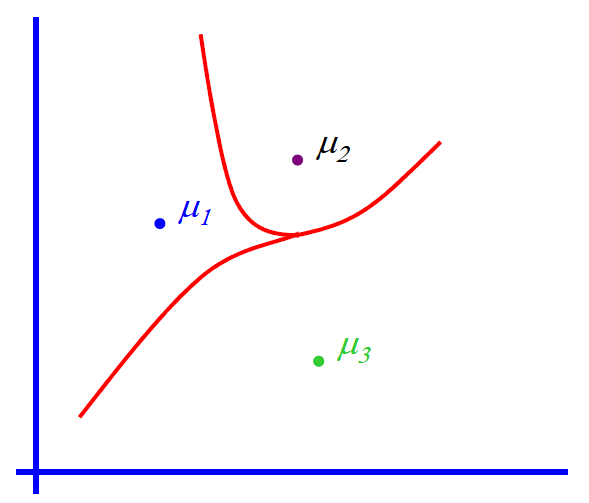
\includegraphics[width=6cm]{pics/general_gmm_2}
"Quadratic Decision boundary"
second-order terms don't cancel out
}
\end{figure}
\end{columns}
\end{frame}

\begin{frame}{GMM: marginal likelihood}
\begin{itemize}
	\item Maximize marginal likelihood:
	\begin{equation} \nonumber
	\begin{aligned}
	&\argmax{} \prod_{j} P(\bm{x}_j) \\
	=&\argmax{} \prod_{j}\sum_{i}^{K}P(y_j=i,\bm{x}_j) \\
	=&\argmax{} \prod_{j}\sum_{i}^{K}P(y_j=i)\textcolor{red}{p(\bm{x}_j|y_j=i)}
	\end{aligned}
	\end{equation}
\end{itemize}
\end{frame}

\begin{frame}{GMM: marginal likelihood}
\begin{itemize}
	\item Uncertain about class of each $\bm{x}_j$ (soft assignment), $P(y_j=i)=P(y=i)$
	\begin{equation} \nonumber
	\begin{aligned}
	&\prod_{j=1}^{N}\sum_{i=1}^{K}P(y_j=i,\bm{x}_j)\propto \\
	&\prod_{j=1}^{N}\sum_{i=1}^{K}P(y=i)\frac{1}{\sqrt{\det(\Sigma_i)}}\exp \left[-\frac{1}{2}(\bm{x}_j-\bm{\mu}_i)^T\Sigma_i(\bm{x}_j-\bm{\mu}_i)\right]
	\end{aligned}
	\end{equation}
	\item How do we find the $\bm{\mu}_i$'s which give max marginal likelihood?
	\begin{itemize}
	\item Set $\frac{\partial F}{\partial \bm{\mu}_i}=0$ and solve for $\bm{\mu}_i$ 's. Non-linear non-analytically solvable.
	\item Use gradient decent: Often slow but doable.
	\end{itemize}
\end{itemize}
\end{frame}

\section{EM Algorithm}
\begin{frame}{Expectation-Maximization (EM)}
\begin{itemize}
\item \textcolor{red}{EM is an optimization strategy for objective functions that can be interpreted as likelihoods in the presence missing data.}
\item It is much simpler than gradient methods.
\item EM is an iterative algorithm with two linked steps:
\begin{itemize}
\item \textcolor{red}{E-step}: fill in hidden values using inference
\item \textcolor{red}{M-step}: apply standard MLE methods
\end{itemize}
\item This procedure monotonically improves the likelihood. Thus it always converges to a local optimum of the likelihood.
\end{itemize}
\end{frame}

\begin{frame}{EM: A simple case}
\begin{itemize}
\item We have unlabeled data $\bm{x}_1, \bm{x}_2, \ldots, \bm{x}_N$
\item We know there are $K$ classes
\item We know $P(y=1), P(y=2),\ldots,P(y=K)$
\item We \textcolor{red}{don't} know $\bm{\mu}_1,\bm{\mu}_2,\ldots,\bm{\mu}_K$
\item We know common variance $\sigma^2$
\end{itemize}
\end{frame}

\begin{frame}{EM: A simple case}
\begin{itemize}
\item Problem formulation:
\begin{equation} \nonumber
\begin{aligned}
&P(data|\bm{\mu}_1\ldots\bm{\mu}_K)\\
=&P(\bm{x}_1\ldots\bm{x}_N|\bm{\mu}_1\ldots\bm{\mu}_K) \\
=&\prod_{j=1}^{N}p(\bm{x}_j|\bm{\mu}_1\ldots\bm{\mu}_K) \qquad \textcolor{red}{Indepentent~data} \\
=&\prod_{j=1}^{N}\sum_{i=1}^{K}p(\bm{x}_j|\bm{\mu}_i)P(y=i) \qquad \textcolor{red}{Marginalize~over~class} \\
\propto&\prod_{j=1}^{N}\sum_{i=1}^{K}\exp\left( -\frac{1}{2\sigma^2}\norm{\bm{x}_j-\bm{\mu}_i}^2 \right)P(y=i)
\end{aligned}
\end{equation}
\end{itemize}
\end{frame}
	
\begin{frame}{Expectation (E) step}
\begin{itemize}
\item IF we know $\bm{\mu}_1,\ldots,\bm{\mu}_K$, then easily compute probability about point $\bm{x}_j$ belongs to class $y=i$
\begin{equation} \nonumber
P(y=i|\bm{x}_j,\bm{\mu}_1,\ldots,\bm{\mu}_K)\propto \exp\left( -\frac{1}{2\sigma^2}\norm{\bm{x}_j-\bm{\mu}_i}^2 \right)P(y=i)
\end{equation}
\end{itemize}
\end{frame}

\begin{frame}{Maximization (M) step}
\begin{itemize}
\item If we know probability about point $\bm{x}_j$ belongs to class $y=i$, then MLE for $\bm{\mu}_i$ is weighted average.
\item Image multiple copies of each $\bm{x}_j$, each with weight $P(y=i|\bm{x}_j)$:
\begin{equation} \nonumber
\bm{\mu}_i = \frac{\sum_{j=1}^{N}P(y=i|\bm{x}_j)\bm{x}_j}{\sum_{j=1}^{N}P(y=i|\bm{x}_j)}
\end{equation}
\end{itemize}

\begin{frmae}{EM for spherical, same variance GMMs}

\end{frmae}

\end{frame}

\end{document}